\subsection{How To Access to the BIOS of the Cincoze}
\label{annex:bios}
You will need to access to the \emph{Basic Input Ouput System} menu
(or BIOS CMOS Setup Utility) to perform some configuration tasks
like set-up the serial port or boot from USB stick. 
To get this acces, turn \emph{OFF} and \emph{ON} the computer, then immediately 
press \textbf{\textless del\textgreater} 
or \textbf{\textless ESC\textgreater}.
You should see a screen similar to the figure
\ref{screen_bios}. If not, you may refer to the
\href{http://www.cincoze.com/data/files/201509/Manual\_DE-1000\_R1.3\_20170621001.pdf}
{User's Manual of the computer}.
\vspace{11pt}

\begin{figure}[!h]
\centering
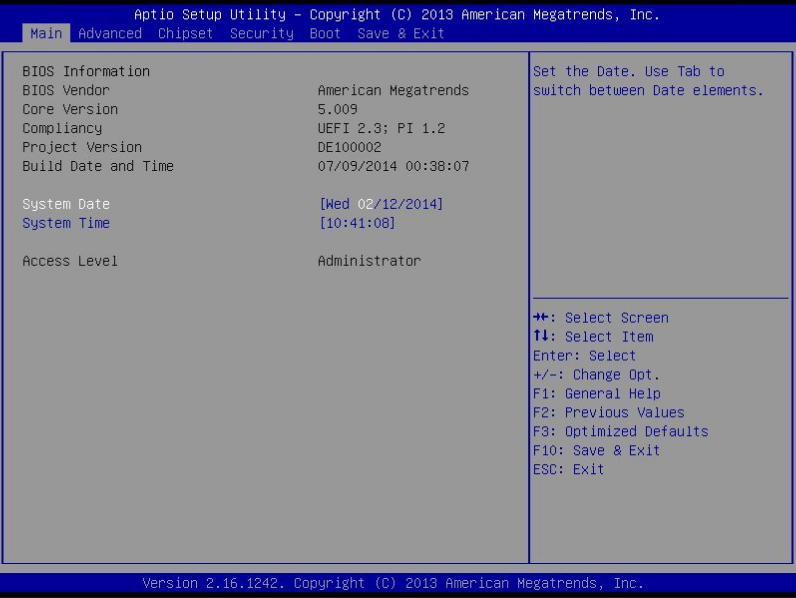
\includegraphics[scale=.43]{images/bios_screenshot.png}
\caption{Screenshot of BIOS}
\label{screen_bios}
\end{figure}

\subsubsection{Pan-Tilt: Serial Port Configuration}
Go to the BIOS (see annex \ref{annex:bios}). Under the tab \emph{Advanced}
go to the menu \emph{Super IO Configuration}, select the serial port for the 
pan-tilt (usually the n°4) and select \emph{RS485 Half Duplex} on the line 
\emph{Onboard Serial Port 4 Mode}. Save and exit. 

